
\documentclass{article}

\usepackage[colorlinks=true,urlcolor=blue,linkcolor=blue]{hyperref}
\usepackage{cleveref}
\usepackage{geometry}
\geometry{a4paper, margin=0.6in}
\usepackage{minted}
\usepackage{graphicx}
\newcommand{\HRule}{\rule{\linewidth}{0.5mm}}
\usepackage{wrapfig}
\usepackage{subcaption}
\usepackage{setspace}
\usepackage{booktabs}
\usepackage[T1]{fontenc}
\usepackage[font=small, labelfont=bf]{caption}
\usepackage[protrusion=true, expansion=true]{microtype}
\usepackage[english]{babel}
\usepackage{sectsty}
\usepackage{url, lipsum}
\usepackage{tcolorbox}
\usepackage{lipsum}
\usepackage[toc,page]{appendix}
\usepackage{charter}
\setlength{\parindent}{1em}
\renewcommand{\baselinestretch}{1.2}

\crefname{appsec}{Appendix}{Appendices}

\usepackage[framemethod=TikZ]{mdframed}
\usepackage{lipsum}
\mdfdefinestyle{MyFrame}{%
    linecolor=blue,
    outerlinewidth=2pt,
    roundcorner=20pt,
    innertopmargin=\baselineskip,
    innerbottommargin=\baselineskip,
    innerrightmargin=20pt,
    innerleftmargin=20pt,
    backgroundcolor=red!20!white}


\newenvironment{myexampleblock}[1]{%
    \tcolorbox[beamer,%
    noparskip,breakable,
    colback=LightGreen,colframe=DarkGreen,%
    colbacklower=LimeGreen!75!LightGreen,%
    title=#1]}%
    {\endtcolorbox}

\newenvironment{myalertblock}[1]{%
    \tcolorbox[beamer,%
    noparskip,breakable,
    colback=LightCoral,colframe=DarkRed,%
    colbacklower=Tomato!75!LightCoral,%
    title=#1]}%
    {\endtcolorbox}

\newenvironment{myblock}[1]{%
    \tcolorbox[beamer,%
    noparskip,breakable,
    colback=white,colframe=DarkBlue,%
    %colbacklower=DarkBlue!75!LightBlue,%
    title=#1]}%
    {\endtcolorbox}


\newenvironment{myitemize}
{ \begin{itemize}
    \setlength{\itemsep}{0pt}
    \setlength{\parskip}{0pt}
    \setlength{\parsep}{0pt}     }
{ \end{itemize}                  }





\begin{document}

\title{ \LARGE \normalsize {The International School of Trigger and Data Acquisition 2018} \vspace{8cm} \\
        \LARGE \textbf{\uppercase{System on Chip Laboratory}} \\ 
        \normalsize \today \vspace*{2\baselineskip}}

\date{}

\maketitle

\begin{figure}[h!]
    \centering
    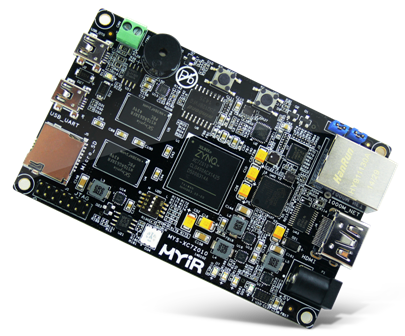
\includegraphics[width=0.7\textwidth]{img/zturn.png}
\end{figure}


\newpage
\tableofcontents
\newpage

%-------------------------------------------------------------------------------
% Section title formatting
\sectionfont{\scshape}
%-------------------------------------------------------------------------------

%-------------------------------------------------------------------------------
% BODY
%-------------------------------------------------------------------------------

\section{Introduction to SoC FPGA}

\subsection{SoC FPGA}

{\color{red}MANU}

The System on Chip(SoC) is getting more and more popular, exceeding the capabilities of a simple microcontroller. SOCs are used mostly in smartphones and tablets due to their low power consumption, much shorter wiring and high level of integration.

This laboratory will thus aim to familiarize you with the \textbf{All Programmable System on Chip (AP SoC)}. The board (presented in Figure \ref{fig:zturnboard}) that you are going to use is called Z-TURN, built around the Xilinx Zynq-7010. It contains an FPGA and a dual-core ARM microcontroller, basically it is a \textbf{System on Chip}.


\begin{figure}[h!]
    \centering
    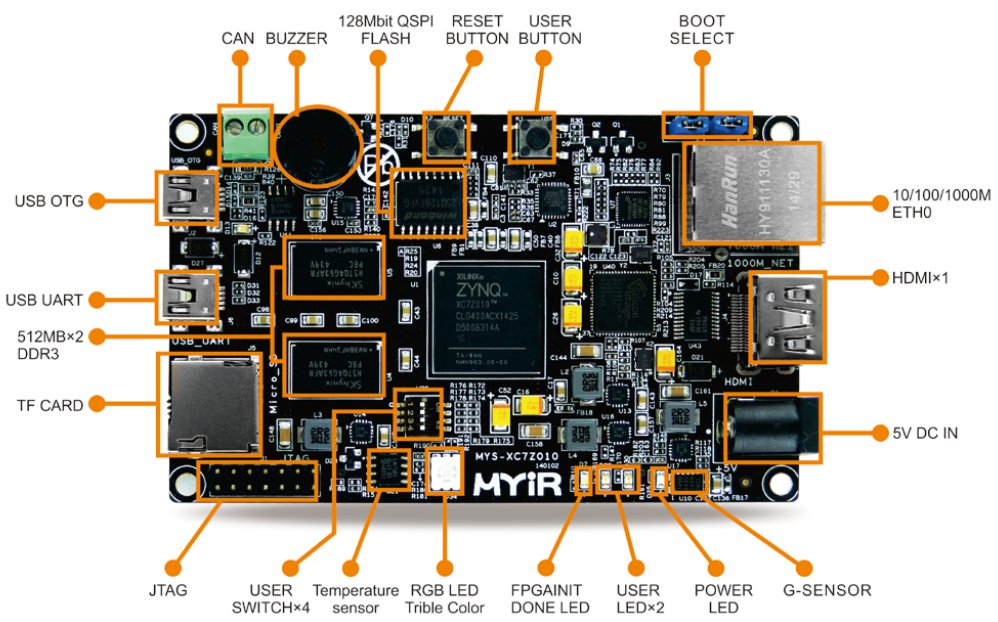
\includegraphics[width=0.9\textwidth]{img/zturn_details.jpg}
    \caption{Z-Turn board capabilities}
    \label{fig:zturnboard}
\end{figure}

After fulfilling this lab, you are mainly going to learn:
\begin{itemize}
\item the workflow of designing an application on FPGA
\item the interaction between an FPGA and an ARM microcontroller
\item getting an overview of the challenges of using this system
\end{itemize}



\subsection{Workflow}




In this laboratory, you will implement the workflow for designing one application used in
High Energy Physics.


ADD MANU's WORK


{\color{red} Explain to the students what is PWM and how does it work to control an LED.}

\subsection{Pulse Width Modulation (PWM) Slave Peripheral for LED control}


In Figure \ref{fig:pwm_waveform}, you can see a basic PWM waveform.  

The FPGA runs at a clock frequency (for this application, we will choose 50 MHz). We can create a PWM waveform  from this clock frequency, by counting a number of clock cycles. There are two important parameters that characterize the PWM waveform: \textbf{the duty cycle} and the \textbf{PWM period}. The PWM  period is set by "waiting/counting" a number of clock cycles,  while the duty cycle  tells us, in one period, how many clock cycles the PWM signal is low.


\begin{figure}[h!]
    \centering
    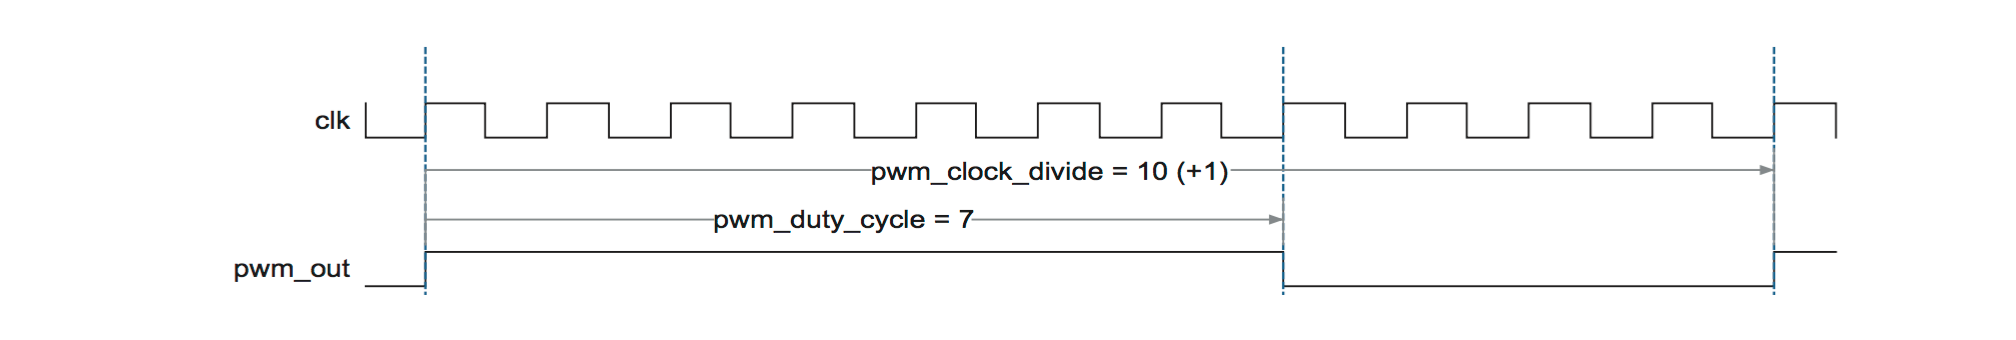
\includegraphics[width=\textwidth]{img/pwm_waveform.png}
    \caption{PWM waveform (Source: Application Note 333, Altera)}
    \label{fig:pwm_waveform}
\end{figure}

Now let's see how we are going to use these two simple parameters to make an RGB LED change its color.


\textbf{RGB LED}

In the case of RGB LED, we need 3 PWMs signals (one per each color), such that the brightness of each of the three LEDs can be controlled independently.

\textbf{\textit{How do we choose the PWM period?}} The driving frequency of the PWM should be fast enough to avoid the flicker effect. A normal human being sees this effect until up to 100 to 150 Hz, so a higher frequency should be better to avoid this effect. For this exercise, we will use a frequency of 1.5 kHz. Let's make some calculations.

The main clock frequency of the FPGA is 50 MHz. We want to use a 1.5 kHz frequency. How much do we need to count?

\begin{equation}
counter = \frac{50000000}{15000} = 30000
\end{equation}

\textbf{\textit{How do we choose the PWM duty cycle?}} The brightness of the LEDs is controlled by the duty cycle. This is up to you to do experiments. You can choose basically any duty cycle in the range of 0$\%$ to 100$\%$.



%\noindent\rule{18cm}{1pt}

\clearpage






\section{Lab Setup}

\subsection{Specifications}
{\color{red}MANU}

HEP TDAQ system


\subsection{Hardware}
{\color{red}MANU}

Front-End board: (ALS-GEVB)
Board with sensor
Back-End board (MYIR Z-turn)
Board with SoC FPGA

\subsection{Gateware}
{\color{red}MANU}

Vivado is used in this part. The gateware is divided in SoC and Fpga fabric parts

SoC

Vivado block schematics


FPGA fabric

HDL language


\subsection{Software}
{\color{red}MANU}

Xilinx SDK is used in this part

Stand-Alone

C++

Embedded Linux 

Very complex, provided by  MYIR


\cleardoublepage
\section{Lab exercises}

\subsection{Hardware assembly}

Connect the board and the laptop.

\begin{myitemize}
\item Ensure that your board is powered on by connecting the Mini-USB to USB cable from computer to the USB\_UART mini-usb socket. This connectivity will also allow us transmit and receive data through serial communication.
\item Connect the programmer on the JTAG port. Make sure the connector matches the pinout from Figure \ref{fig:board_pinout}.
\end{myitemize}

 \begin{figure}[h!]
    \centering
    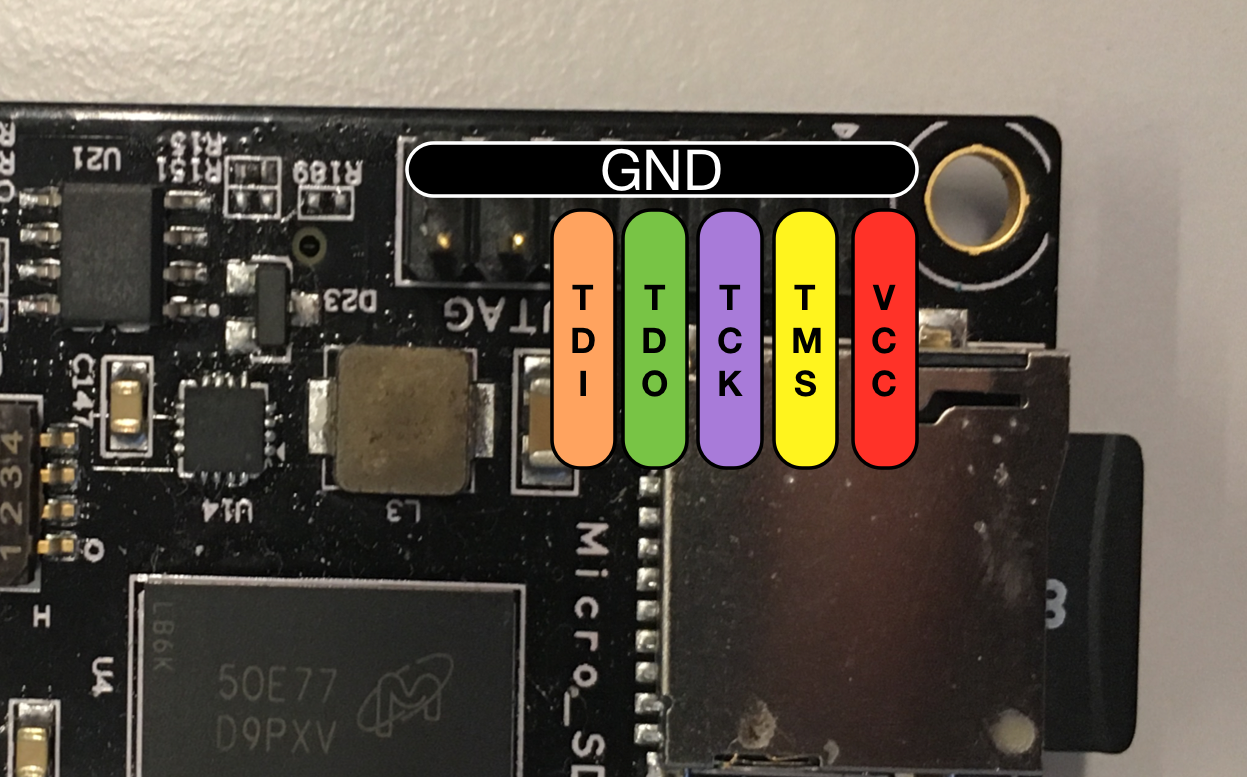
\includegraphics[width=0.4\textwidth]{img/boardpinout.png}
    \caption{JTAG Pinout}
    \label{fig:board_pinout}
\end{figure}


\subsection{Gateware development}

\subsubsection{Project Setup}

\begin{enumerate}
\item Open an Ubuntu terminal(CTRL-T) and type the following to launch Vivado Design Suite.
    \begin{tcolorbox}
    \begin{minted}{c}
    vivado &
    \end{minted}
    \end{tcolorbox}


\item Create a new project and call it \textbf{detector}.

Click \textbf{Next} and tick \textbf{RTL Project}. 
Next, you will be asked to add sources to your design. For the moment, we will keep the project empty. However, we need to specify \textbf{VERILOG} for both \textit{Target Language} and \textit{Simulator Language}. Press \textbf{Next}, and you will be asked about Existing IP and Constrains files. Keep them both empty.

\item Choose the hardware platform where we will run the applications. 

The development board is entitled MYS-7Z010-C-S Z-turn (Figure \ref{fig:board}).  Press \textbf{Next} and then \textbf{Finish}.  

\begin{figure}[h!]
    \centering
    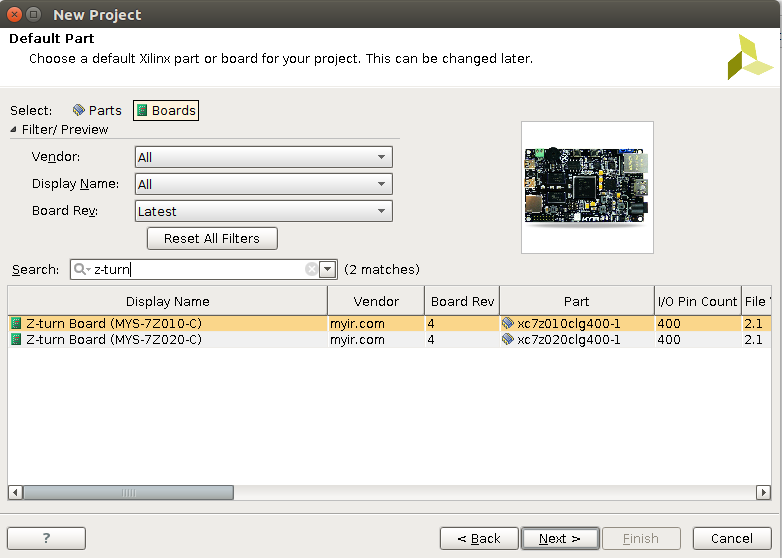
\includegraphics[width=0.5\textwidth]{img/00_Board.png}
    \caption{Hardware Selection}
    \label{fig:board}
\end{figure}


The starting page of the project should like in Figure \ref{fig:first_page}. In this project, we will implement the necessary files to control an RGB LED.


\begin{figure}[h!]
    \centering
    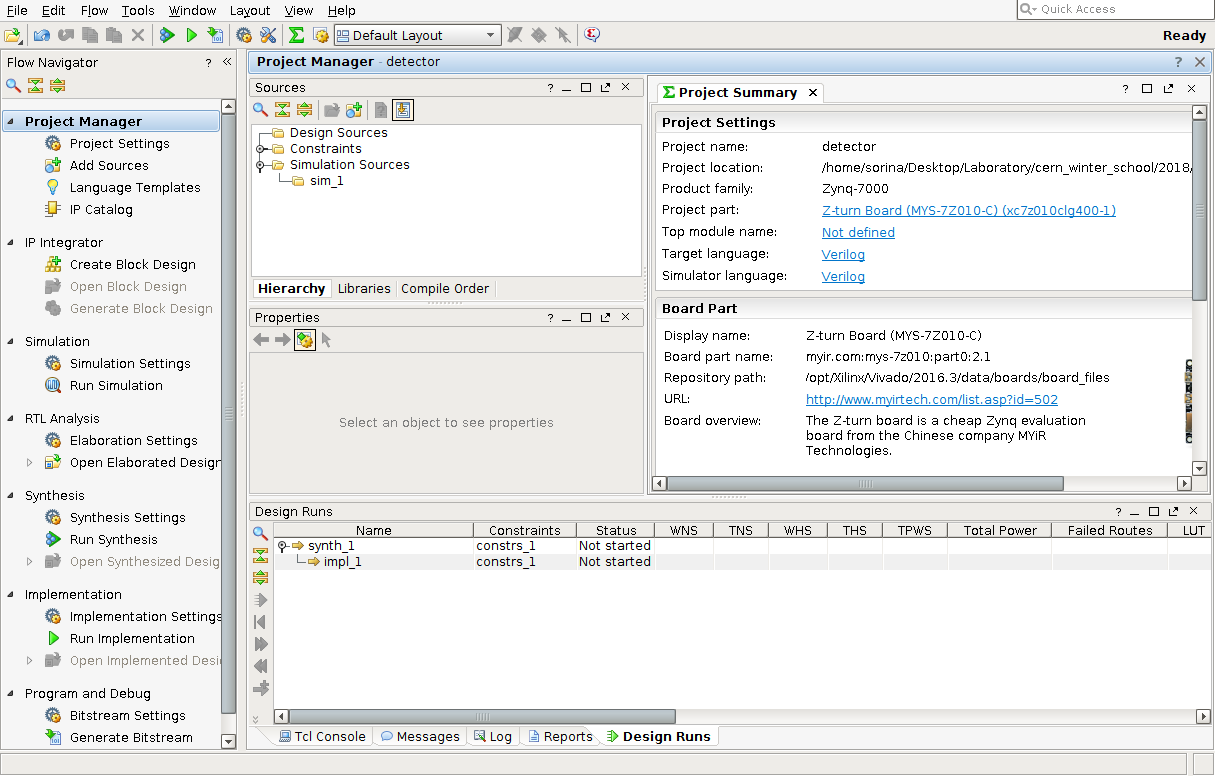
\includegraphics[width=0.7\textwidth]{img/01_Project_Structure.png}
    \caption{Initial Project Structure}
    \label{fig:first_page}
\end{figure}

\end{enumerate}



\subsection{Block Design for SOC}

\begin{enumerate}


\item Create the Block Design

On the left of the window, in the \textbf{Flow Navigator}, choose \textbf{Create Block Design} and call it \textbf{detector}. 
% The environment should look like in Figure \ref{fig:diagram_second_page}.

% \begin{figure}[h!]
%     \centering
%     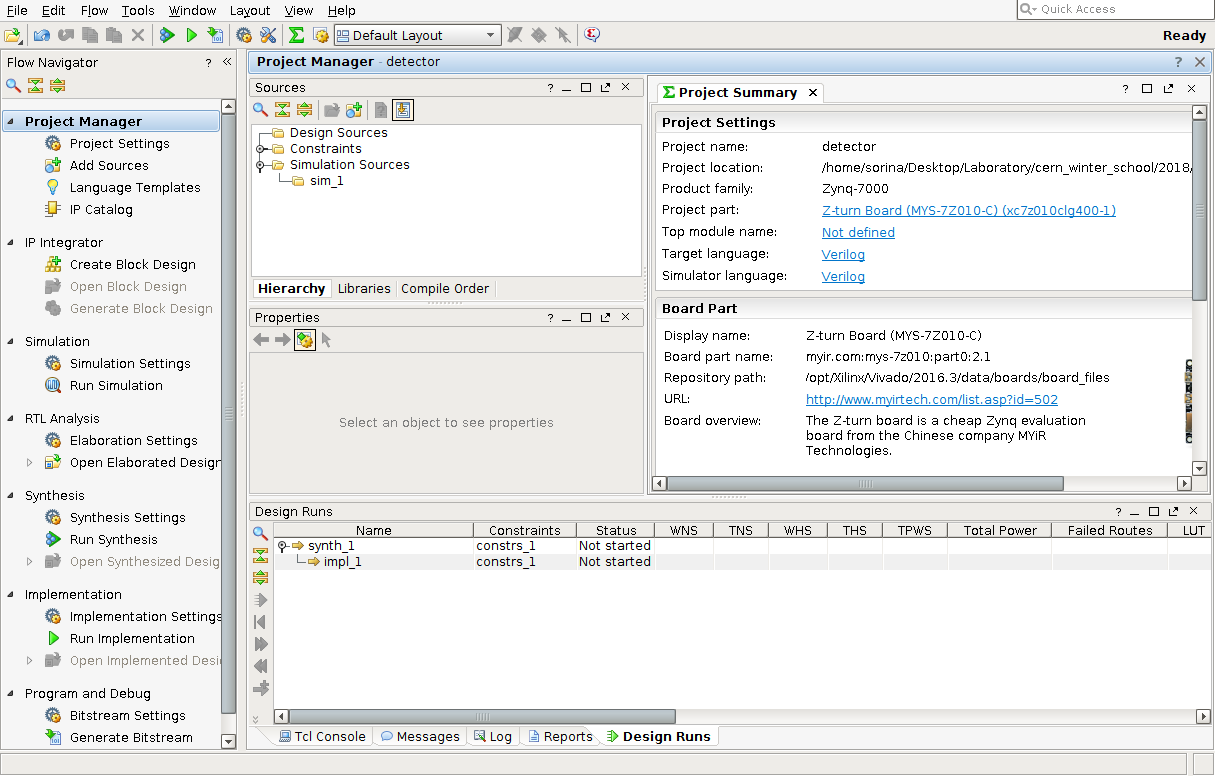
\includegraphics[width=0.7\textwidth]{img/01_Project_Structure.png}
%     \caption{Block Diagram Project Structure}
%     \label{fig:diagram_second_page}
% \end{figure}



\item Define SoC with the wizard

Press \textbf{Add IP} 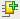
\includegraphics[width = 0.5cm]{img/icon_add.png} and choose \textbf{Zynq7 Processing System}. Click {\color{blue}\underline{Run Block Automation}} to auto-configure it. Double click on it to open the wizard.

\item Discuss with your tutor the structure of the System on Chip. We will leave most of the settings as default, apart from several.

\begin{itemize}
    \item Click on PS-PL Configuration -> HP Slave Axi Interface and De-select S AXI HPO INTERFACE (Figure \ref{fig:Zynq_Wizard} a))
    \item Click on Peripherals I/O Pins and leave ticked only the peripherals which we are using (Figure \ref{fig:Zynq_Wizard} b):
    
        \begin{itemize}
            \item UART1 - for communication
            \item I2C1 - for interface with the Light Sensor
        \end{itemize}
    \item Clock Configuration. Select only FCLK\_CLK0 and change its value to 50 MHz. (Figure \ref{fig:Zynq_Wizard} c)
\end{itemize}

\begin{figure}[h!]
    \centering
    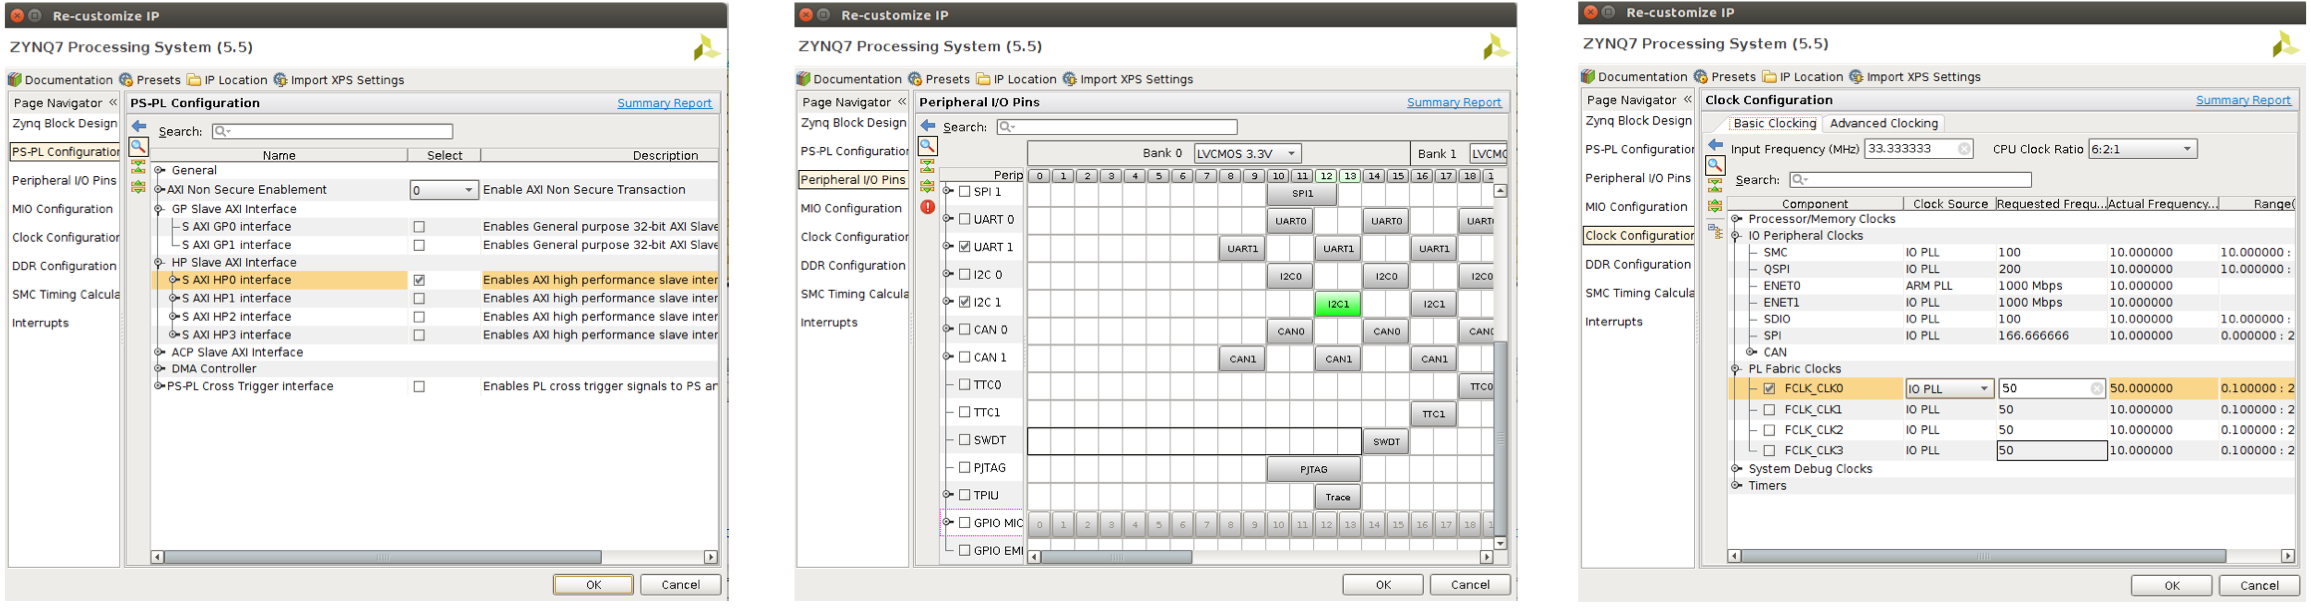
\includegraphics[width=\textwidth]{img/04_wizzard_zynq.png}
    \caption{Zynq Wizard a)PS-PL Configuration b) Peripherals c)Timing }
    \label{fig:Zynq_Wizard}
\end{figure}



\end{enumerate}




\subsection{Block Design for FPGA Fabric}

\begin{enumerate}

\item Add the PWM IP module to the project

The PWM IP was already implemented for you, but you need to add it to the library. Click on the \textbf{IP settings} icon 
\includegraphics[width = 0.5cm]{img/settingsicon.png}.
 Choose \textbf{Repository Manager} from the upper tabs. Click on $+$ symbol and add the content found at the following path relative to your main folder:
 
 \textit{/ip/pwm\_verilog\_1.0}



Now the PWM folder is added to your project so you can choose it from the IP Library. Press \textbf{Add IP} 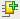
\includegraphics[width = 0.5cm]{img/icon_add.png} and type "pwm".


\item Let's dig into how the PWM Peripheral was designed

Right click on the \textbf{pwm\_verilog\_v1 IP} and select \textbf{Edit in IP Packager}. Another project (Figure \ref{fig:ip}) that contains the files written by the tutors for this IP will open.  In the Source part, you will see an hierarchical design in Verilog. 
The top level is called \textit{pwm\_verilog\_v1\_0.v} and contains an instantiation of the  \textit{pwm\_verilog\_v1\_0\_S00\_AXI.vhd} where the logic is implemented. If you open  \textit{pwm\_verilog\_v1\_0\_S00\_AXI.v}, you will see the implementation of PWM code outlined by the following comments:



\begin{minted}{vhdl}
 -- User to add parameters/ports/logic here
 ...
 -- User parameters/ports/logic ends
\end{minted}

\noindent\rule{16.5cm}{1pt}

\noindent\begin{minipage}{.1\textwidth}
  \centering
  
\includegraphics[height=1cm]{img/talking_icon.png}
\end{minipage}
\begin{minipage}{.8\textwidth}
\hspace{0.2cm} Discuss the code with the tutor.
\end{minipage}%

\noindent\rule{16.5cm}{1pt}


\begin{figure}[h!]
    \centering
    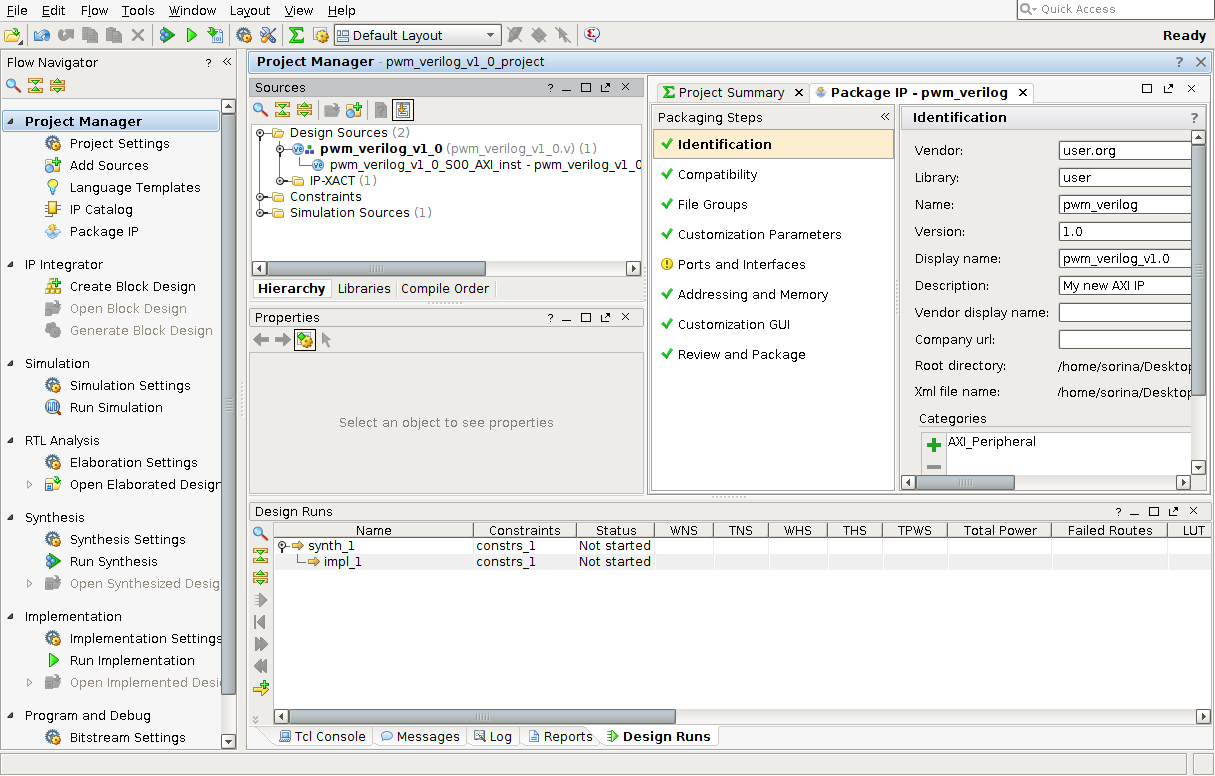
\includegraphics[width=0.85\textwidth]{img/05_PWM_IP.png}
    \caption{PWM IP Project Structure}
    \label{fig:ip}
\end{figure}










\item Connect the PWM controller HDL module to the SoC


We need to create PWM outputs, in order to connect them to our SoC. Click on each PWM output and press CTRL-K or \textbf{Create Port} from the Menu. (Figure \ref{fig:port_creation}) Do so for all the 3 ports.


\begin{figure}[h!]
    \centering
    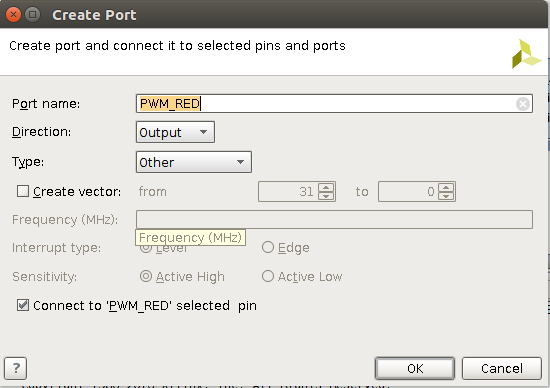
\includegraphics[width=0.4\textwidth]{img/05_CreatePort.png}
    \caption{Port Creation for each PWM output}
    \label{fig:port_creation}
\end{figure}


Right now, both systems should look like in Figure \ref{fig:both_ips}.

 \begin{figure}[h!]
\centering
  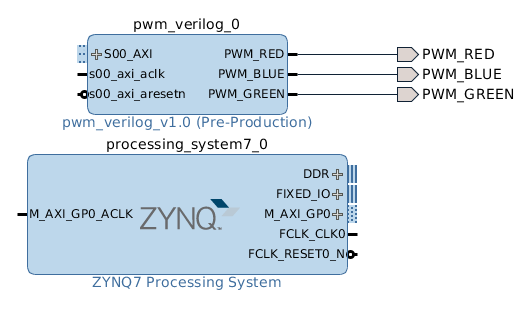
\includegraphics[width=0.6\linewidth]{img/03_BothIPs.png}
  \caption{Both IPs}
  \label{fig:both_ips}
\end{figure}


Last step is to choose {\color{blue} \underline{Run Connection Automation}}, let the settings as default, press OK and let the Designer Assistance to do this work on your behalf. The window should now look similar to Figure \ref{fig:block_diagram_system}. However, the Design Assistant is placing the blocks in a not-very-organized way. For a better view, we advise you to click on the Regenerate Design button 
\includegraphics[width = 0.5cm]{img/icon_refresh.png} in the right Menu. Looks better, right?


\noindent\rule{16.5cm}{1pt}

\noindent\begin{minipage}{.1\textwidth}
  \centering
  
\includegraphics[height=1cm]{img/talking_icon.png}
\end{minipage}
\begin{minipage}{.8\textwidth}
\hspace{0.2cm} Discuss the block diagram with your tutor.
\end{minipage}%

\noindent\rule{16.5cm}{1pt}




\begin{figure}[h!]
    \centering
    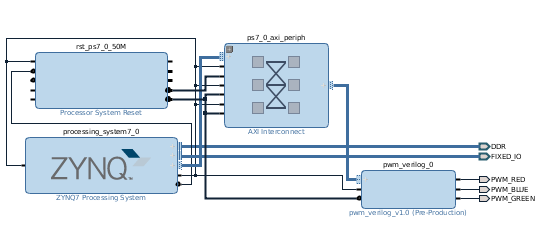
\includegraphics[width=0.85\textwidth]{img/06_BlockReady.png}
    \caption{Block Diagram of our System}
    \label{fig:block_diagram_system}
\end{figure}



\end{enumerate}


\subsection{Synthesis, Implementation \& Static timing analysis}


\noindent\rule{16.5cm}{1pt}

\noindent\begin{minipage}{.1\textwidth}
  \centering
  
\includegraphics[height=1cm]{img/talking_icon.png}
\end{minipage}
\begin{minipage}{.8\textwidth}
\hspace{0.2cm} Discuss with your tutor the differences between Synthesis, Implementation and Bistream generation for an FPGA.
\end{minipage}%

\noindent\rule{16.5cm}{1pt}

\begin{enumerate}


\item Create Wrapper

From the block design, we need to create the Verilog code. Therefore, in the Project Sources - Design Sources, you will right click on the \textbf{detector.bd} and select \textit {Create HDL Wrapper}. Let the default option and press OK. Now the VHDL Wrapper should have been created. Verify that the signals PWM\_RED, PWM\_BLUE and PWM\_GREEN appear instantiated. 


\begin{figure}[h!]
    \centering
    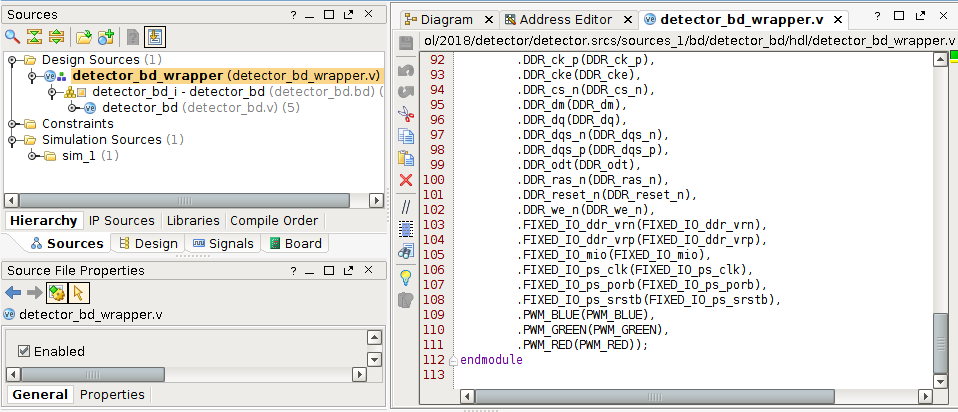
\includegraphics[width=0.85\textwidth]{img/16_wrapper_instantiated.png}
    \caption{Wrapper with the PWM outputs instantiated}
    \label{fig:block_diagram_system}
\end{figure}


 \item Create Constraint File
 
The Constraint File is used in the implementation phase. After the synthesis will be run, and the available top-level nets are "known", they will be matched to the "real" pins.
  
Right click on the Constraints directory and click \textbf{Add Source} (Add or Create Constraints). The constraints file are present in \textit{/constraints/} directory.
Open it and check it together with the tutor


\item Generate the bitstream 

The last step in FPGA design is the generation of the bitstream.
To generate the bitstream, look into the Flow Manager on the left of the screen and press \textbf{Generate Bitstream (Figure \ref{fig:export_hardware_generate_bitstream})}. You will need to wait a bit longer until the bitstream is created. Check for errors in the process and solve them. 

\item Export the hardware
Now, that the bitstream was successfully created, we need to export the hardware such as we can use it together with the ARM dual-core microcontroller. 

To export the hardware, press \textbf{File $>$ Edit $>$ Export $>$ Export Hardware}. Tick \textit{Include bitstream} like in Figure \ref{fig:export_hardware_generate_bitstream}.


 \begin{figure}[h!]
\centering
\begin{minipage}{.425\textwidth}
  \centering
  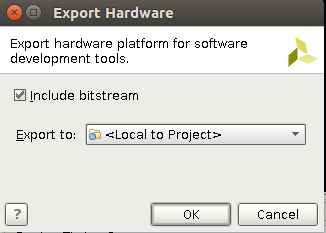
\includegraphics[width=0.8\linewidth]{img/export_hardware.png}
\end{minipage}%
\begin{minipage}{.425\textwidth}
  \centering
  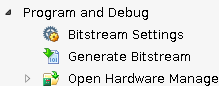
\includegraphics[width=0.8\linewidth]{img/generate_bitstream.png}
\end{minipage}
\caption{a) Export Hardware Window b) Generate Bitstream in Flow Manager}
\label{fig:export_hardware_generate_bitstream}
\end{figure}

\end{enumerate}


\section{Software development}

\begin{enumerate}
\item Create the BSP

In Vivado, press \textbf{File $>$ Launch SDK}. Now, the hardware shall be automatically imported in Xilinx SDK and you can create a software application (Figure \ref{fig:sdk_first_page}).

From now on, we will create the link between the FPGA and the dual-core ARM microcontroller. In our case, the ARM microcontroller is used to read the detector sensor and send signals to the FPGA fabric that further controls an RGB LED.

\item Create a New Application Project

Select \textbf{File -> New -> Application Project}. Select Empty Application and call it \textbf{detector\_controller}.


\item  Add the Cpp file

Some files were already written to make your life easier, such as the driver to read the light detector through I2C. 

In the \textbf{Project Explorer}, go to folder \textit{detector\_controller/src} and add the source files available in \textbf{sw} folder.


\item  Modify the Cpp file

Open the \textbf{main.c}. Read the instructions and solve the simple state machine.

\begin{minted}{c}
        /*
         * i2c_getDataDetector(IIC_DEVICE_ID) returns the value
         * read by the sensor as an integer
         *
         * Xil_Out32(COLOR, brightness) sets the color of the LED
         * from 0 to MAX_BRIGHTNESS
         *
         *  xil_printf("%d", value) prints an integer using UART
         */

        /* Write your code here
         * Implement a state machine that turns on the RED LED
         * when the value exceeded certain threshold
         *
         * Otherwise, make the BLUE LED's brightness follow the sensor
         * readout (e.g. brightness = x*sensor_value
         *
         * Print the sensor_value
         */
\end{minted}



\item  Execute the code on the SoC FPGA

Ask your tutor for help in running the application and programming both the FPGA and the microcontroller.

\item  Verify the results

\begin{figure}[h!]
    \centering
    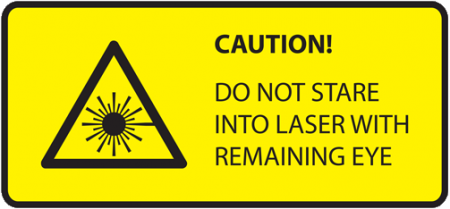
\includegraphics[width=0.4\textwidth]{img/laser.png}
    \label{fig:block_diagram_system}
\end{figure}

\end{enumerate}

\section{Embedded Linux}
\begin{enumerate}
\item  Insert the SD card with the file system on the slot of the Z-turn

\item Find Jumper 1 and Jumper 2 (JP1 and JP2) and make sure they are in the following order:
\begin{minted}{c}
JP1 OFF 
JP2 ON
\end{minted}


\item Execute the program

To run the webserver, you need to type in the emulator the following:

   \begin{tcolorbox}
        \begin{minted}{c}
bokeh serve --host 192.168.2.2:5006 read_event.py
        \end{minted}
    \end{tcolorbox}

Then, in your host computer, open a webbrowser and type the IP, as seen in Figure \ref{fig:bokeh}.

\begin{figure}[h!]
    \centering
    
\includegraphics[width=0.6\textwidth]{img/bokeh.png}
    \caption{Host address}
    \label{fig:bokeh}
\end{figure}

\item Check the webserver and verify the results
\end{enumerate}


Then, the plot will be displayed interactively! Have fun!

\begin{figure}[h!]
    \centering
    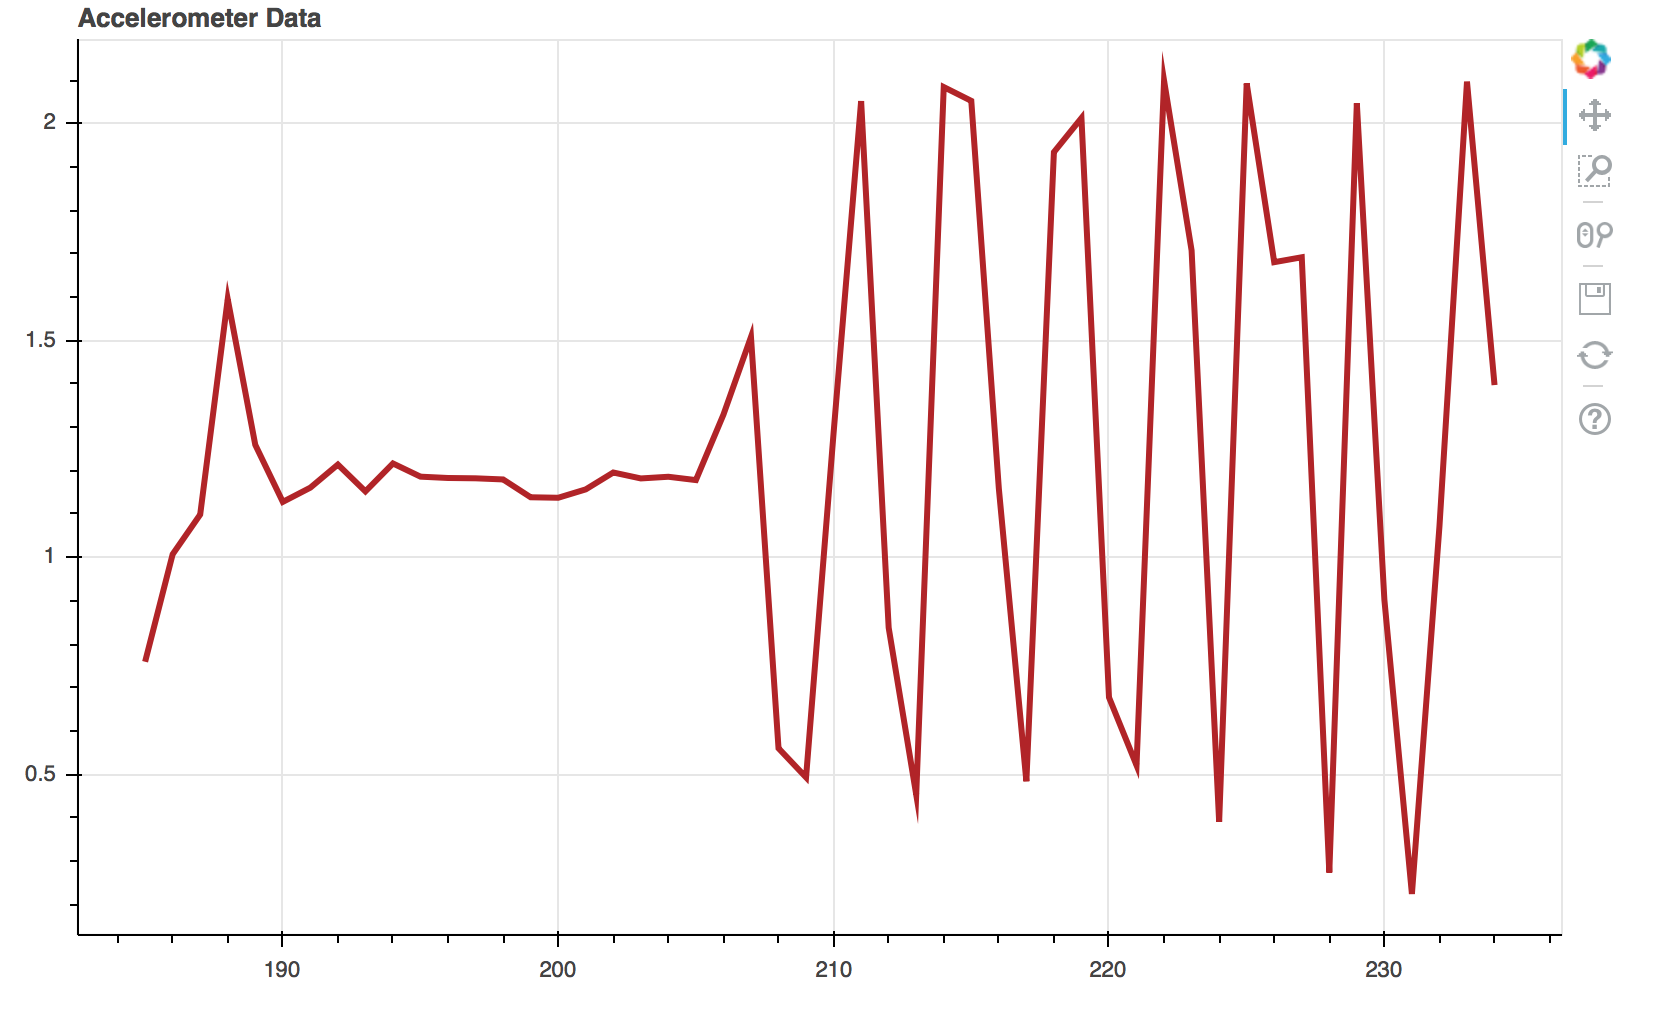
\includegraphics[width=0.6\textwidth]{img/acc.png}
    \caption{Host address}
    \label{fig:bokeh}
\end{figure}


Now you can play with the setup and discuss about it with the tutor


%  \begin{figure}[h!]
%     \centering
%     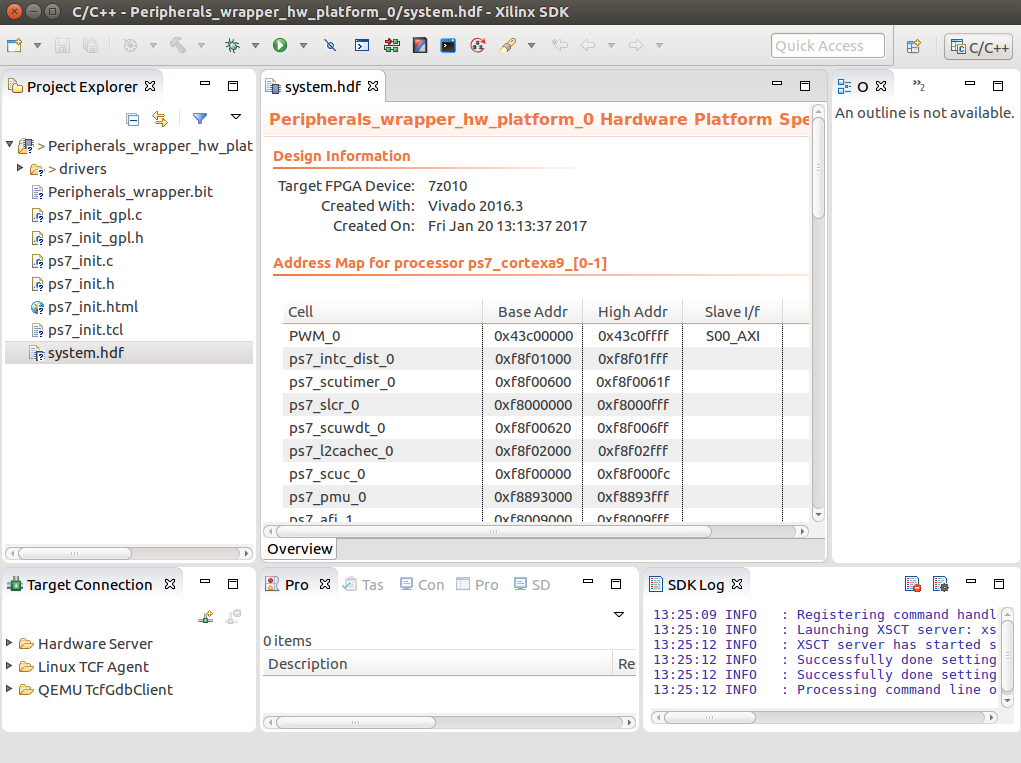
\includegraphics[width=0.85\textwidth]{img/xsdk_first_page.png}
%     \caption{XSDK First Page after bitstream was exported}
%     \label{fig:sdk_first_page}
% \end{figure}



%  \item Our first "Hello World Application"

% Select \textbf{File $>$ New $>$ Application Project}.

% The New Project dialog box opens. As Project Name, type the name desired, for example
% \textit{LED\_Buzzer\_Controller} (Figure \ref{fig:start_proj_xsdk}). Press \textbf{Next}. From the Available Templates, choose \textit{"Hello World"}. 

% Click \textbf{Finish}. 


%  \begin{figure}[h!]
% \centering
% \begin{minipage}{.425\textwidth}
%   \centering
%   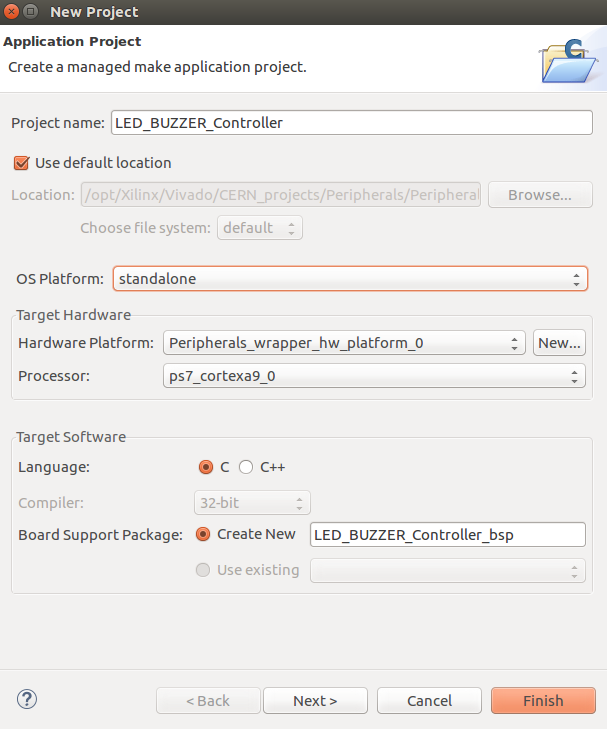
\includegraphics[width=0.8\linewidth]{img/app_project.png}
% \end{minipage}%
% \begin{minipage}{.425\textwidth}
%   \centering
%   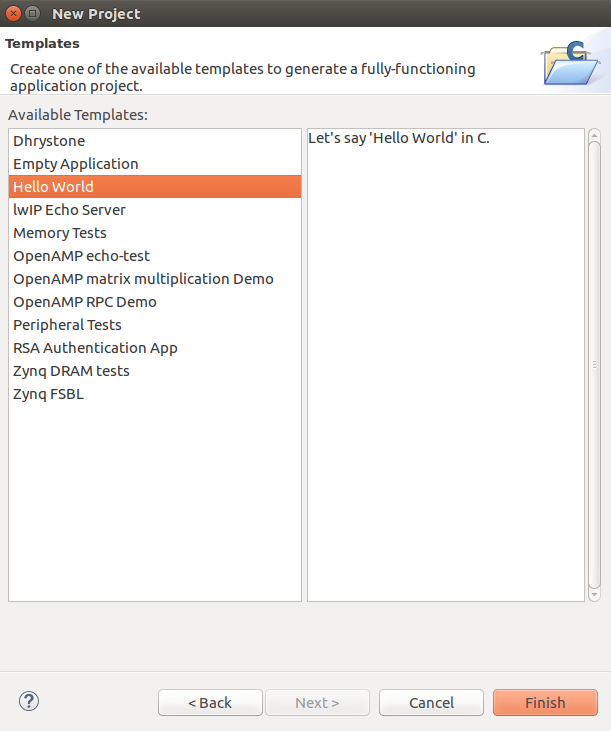
\includegraphics[width=0.8\linewidth]{img/hello_world.png}
% \end{minipage}
% \caption{Starting a project in XSDK}
% \label{fig:start_proj_xsdk}
% \end{figure}


% In the top menu choose

% Project -> Building Configurations -> Set Active -> Release


% \item Connect the board

% To run the first application, you need to do the following simple steps on the hardware site:
% \begin{myitemize}
% \item Ensure that your board is powered on by connecting the Mini-USB to USB cable from computer to the USB\_UART mini-usb socket. This connectivity will also allow us transmit and receive data through serial communication.
% \item Connect the programmer on the JTAG port. Make sure the connector matches the pinout from Figure \ref{fig:board_pinout}.

 
%  \begin{figure}[h!]
%     \centering
%     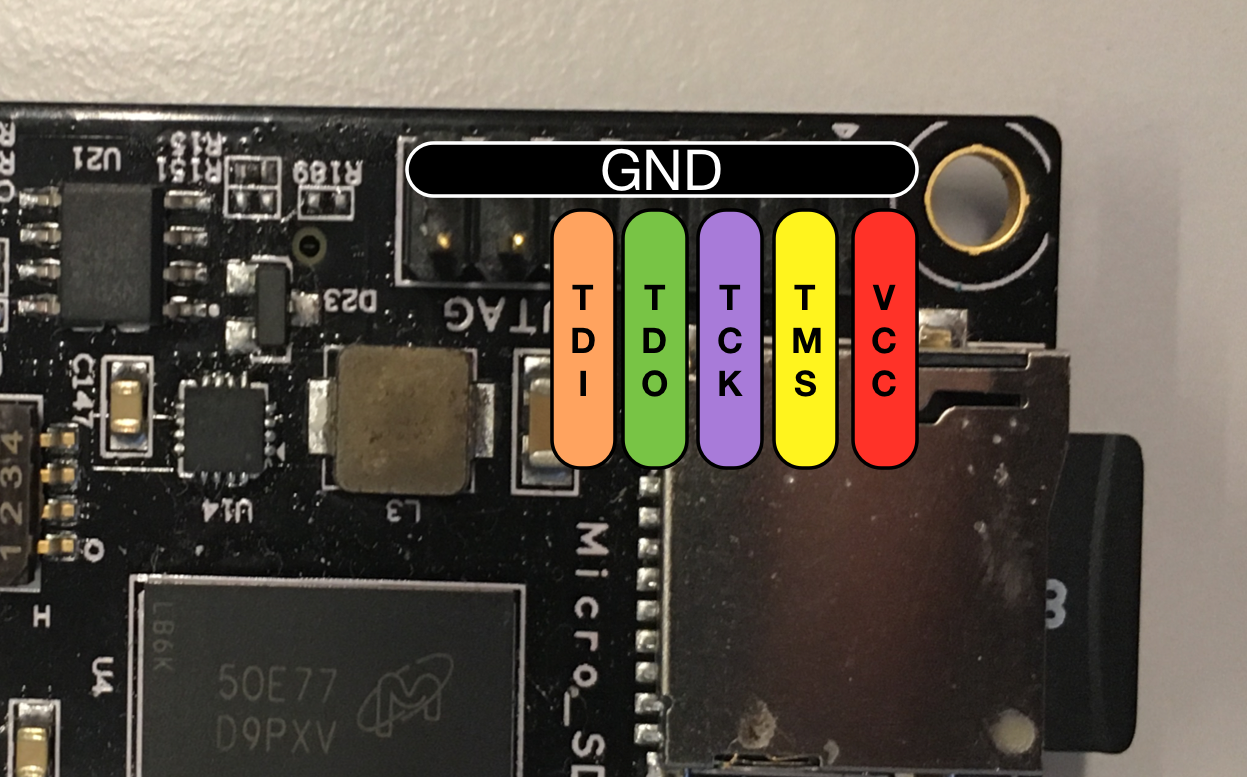
\includegraphics[width=0.4\textwidth]{img/boardpinout.png}
%     \caption{JTAG Pinout}
%     \label{fig:board_pinout}
% \end{figure}


% \end{myitemize}

% \item Run the first application

% Open the project source files (in the \textbf{src} folder), and double-click on the helloworld.c. 
% In that file, add the next sequence before the printing line of code. In this way, you will see the output running all the time on the terminal.

% \begin{minted}{c}
% while(1)
% \end{minted}

% Find the following icon to build the project 
\includegraphics[width = 0.6cm]{img/run/build.png} and click on the downward arrow. Make sure the Release version is selected and then build it. Verify that the build is successful.



% Next, we need to setup the programming chain, as firstly the FPGA is programmed (bitstream loaded) and then the application is loaded (.elf file).



% Go into \textbf{Run > Run configurations} and do the settings from Figures \ref{fig:run_part1} and \ref{fig:run_part2} below:

%  \begin{figure}[h!]
%     \centering
%     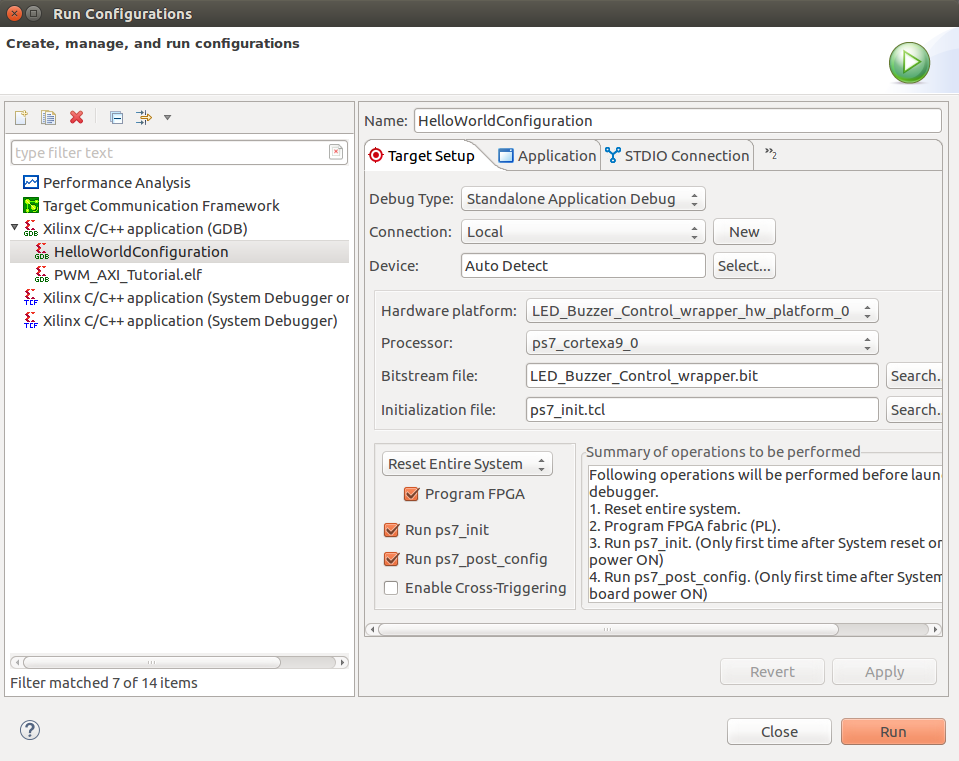
\includegraphics[width=0.7\textwidth]{img/run/run_part1.png}
%     \caption{Target Setup}
%     \label{fig:run_part1}
% \end{figure}

%  \begin{figure}[h!]
%     \centering
%     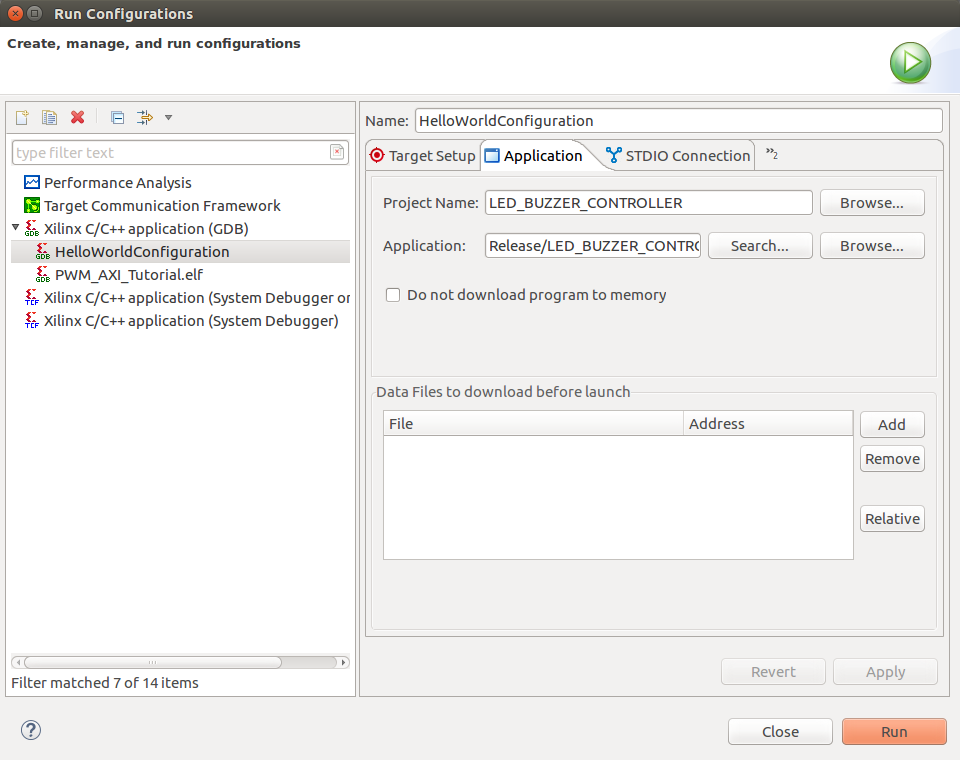
\includegraphics[width=0.7\textwidth]{img/run/run_part2.png}
%     \caption{Application Setup}
%     \label{fig:run_part2}
% \end{figure}

% Wait until the system is configured and programmed.

% \item See the output

% Open a terminal \textbf{CTRL+ALT+T} and open the picocom terminal as following: 

% \begin{tcolorbox}
% \begin{minted}{c}
% picocom -b 115200 /dev/ttyUSB0
% \end{minted}
% \end{tcolorbox}

% Make sure you put the correct serial device "ttyUSBX", according to your system.

% Now, you shall see a long list of "Hello World!"

% \item Let's run a more complex application.

% At the beginning of this laboratory, we presented two applications we are going to implement. For simplicity, we provided you with the source code for this application that can be seen in the Laboratory folder or in Appendix \ref{appendix:C}. You just need to run it and understand the code. 


% The source code contains two $*.c$ files and two header files.


% $itoa_fcn.c$ - contains utility function used to convert a number to a string to be sent to UART using "print" function

% $main.c$ - contains the main logic of the programme


% To run it, firstly, you need to delete the \textit{helloworld.c}. Then, select the \textit{src} folder, and import the aforementioned code by right click and selecting \textbf{Import > General > File System}. Add the Laboratory folder like in Figure \ref{fig:import}.

%  \begin{figure}[h!]
%     \centering
%     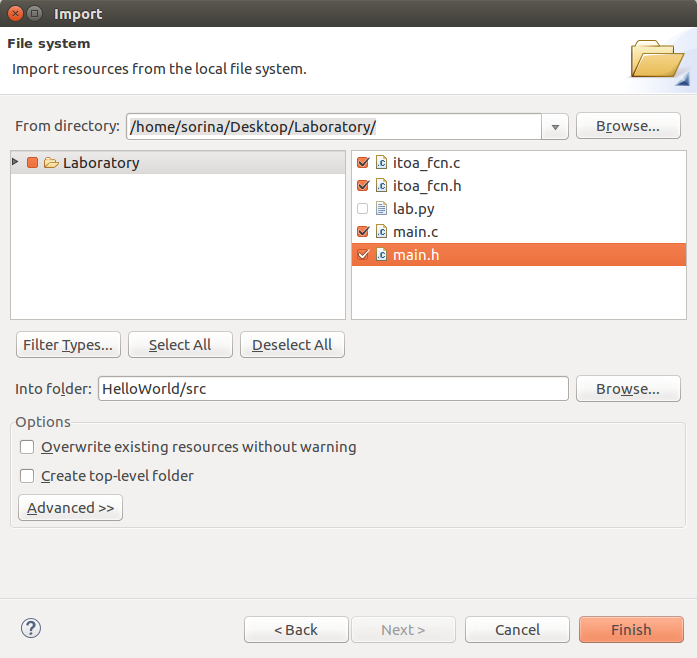
\includegraphics[width=0.7\textwidth]{img/run/import.png}
%     \caption{Import source files}
%     \label{fig:import}
% \end{figure}

% Now, run the application similarly and HAVE FUN! (before moving to the LINUX part)

% \end{enumerate}



% \clearpage

% \section{LINUX OS on System on Chip}


% \subsection{Introduction}

The current kit comes with Ubuntu 12.04 installed on a MicroSD card. Using this 
operating system, we will read the accelerometer data from the ADXL346 accelerometer
already mounted on board. This data will be feed into \textbf{bokeh}, which is a Python interactive visualization library which will also act as a server. In addition,
a control system will be added such as when the acceleration exceeds a certain treashold, a buzzer will start buzzering and an LED will turn red.

In real life, you can use this type of application to detect the high accelerations the astronauts are exposed during training and trigger a warning sound and light when certain threashold is exceeded.


\subsubsection{How is LINUX OS interacting with both the accelerometer and the buzzer?}

The I/O subsystem is the part of the Linux kernel that manages the various devices such as keyboards and mouse, devices usually used by any users. On top of this, it comes the Industrial I/O subsystem (IIO) that are analog to digital or digital to analog convertors, for example \textbf{the accelerometer, gyroscopes, proximity sensors} with the aim to extend the I/O subsystem. A typical device falling into the IIO category would be connected via SPI or I2C.




\subsubsection{How is LINUX OS interacting with the LEDs?}


\subsection{Let's get started!}

Now, we will move on with running an operating system on the System on Chip. For this, we will do the following steps:
\begin{myitemize}
\item you disconnected the JTAG cable used previously to programme the board
\item the mini SD Card is inserted in its socket
\item find Jumper 1 and Jumper 2 (JP1 and JP2) and make sure they are in the following order:
\begin{minted}{c}
JP1 OFF 
JP2 ON
\end{minted}
\end{myitemize}


When previously steps are done, you will see the RGB LED blinking on the board. It is very
important to make these configurations before moving on to the next section of the lab.

\subsection{Further configurations}

The SD card contains the image of Ubuntu 12.04 and will boot it on the board at every restart.

\subsubsection{Screen}

\subsubsection{File transfer between host computer and the board}

% Connect a screen to see that it works

% Open a terminal and communicate 

% Send a file through SSH

\subsection{Interact with the RGB LED and the Buzzer}




\subsection{Webserver}
Now, we will learn how to display the accelerometer values on an webserver running
on the host computer.



 %Each device provides one or more /dev/input/eventN nodes that a process can interact with. For example  reading events from the device.


 %The events themselves are in the form of struct input_event, defined in linux/input.h and consist of a event type (relative, absolute, key, ...) and an event code specific to the type (x axis, left button, etc.).

 %Any event coming from the physical hardware goes into the kernel's input subsystem and is converted to an evdev event that is then available on the event node.






% \clearpage

% \begin{appendices}
% \crefalias{section}{appsec}
% \section{Setting up the picocom terminal}
% \label{appendix:graph}
% \begin{myitemize}
    \item Install Picocom:

    \begin{tcolorbox}
        \begin{minted}{c}
        sudo apt-get install picocom
        \end{minted}
    \end{tcolorbox}

    \item Find the device dev path for the board:

    \begin{tcolorbox}
        \begin{minted}{c}
        dmesg | grep tty
        \end{minted}
    \end{tcolorbox}

    \item Give permission to users to write and read, presuming that the device dev path is ttyUSB0

    \begin{tcolorbox}
        \begin{minted}{c}
        sudo chmod 666 /dev/ttyUSB0
        \end{minted}
    \end{tcolorbox}

    \item Start picocom with a baudrate of 115200 

    \begin{tcolorbox}
        \begin{minted}{c}
        picocom -b 115200 /dev/ttyUSB0
        \end{minted}
    \end{tcolorbox}

    \item To exit Picocom: CTRL-A and CTRL-X


\end{myitemize}


% \clearpage
% \section{Connecting the board to a network}
% \label{appendix:b}
% \begin{myitemize}
\item{Get the board connected to Internet} 

To be able to get the board connected to the Internet, you need to use the laptop as a NAT box. This is done by enabling “Share internet connection via ethernet port” on the laptop. The (only) ethernet interface of the laptop is connected to the board. The connection to the internet is done through the wireless (which should not have 802.1x enabled).



On the side of the board, we configure the network adaptor in the file /etc/network/ interfaces as following:
    \begin{tcolorbox}
    \begin{minted}{c}
    auto eth0
    iface eth0 inet static
    address 192.168.2.2
    netmask 255.255.255.0 gateway 192.168.2.1 dns-nameservers 192.168.2.1
    \end{minted}
    \end{tcolorbox}

After adding these lines to the file, the network stack must be started: 

\begin{tcolorbox}
    \begin{minted}{c}
    service networking start
    \end{minted}
\end{tcolorbox}

(this will also be done automatically at boot time).


\item{Test the network by running:}


\begin{tcolorbox}
    \begin{minted}{c}
    apt-get update
    ping 8.8.8.8
    \end{minted}
\end{tcolorbox}


\item{Getting ssh to work}

A bit more conveniënt way to have a terminal connection is directly over the network with ssh. This makes the installation of ssh necessary on the board:


\begin{tcolorbox}
    \begin{minted}{c}
    apt-get install ssh
    \end{minted}
\end{tcolorbox}

Next , set the root password with the "passwd" command.
Now, from the NAT host (i.c. your laptop), it is possible to connect though ssh:


\begin{tcolorbox}
    \begin{minted}{c}
    ssh -l root 192.168.2.2 
    \end{minted}
\end{tcolorbox}

The output will be : 


    \begin{minted}{c}
    root@localhost:~#
    \end{minted}

\end{myitemize}







% \clearpage
% \section{Cheating Sheet - Final Code for FPGA PART}
% \label{appendix:C}
% \textbf{main.c}
\begin{minted}{c}
#include "xparameters.h"
#include "xil_io.h"
#include "stdlib.h"
#include "itoa_fcn.h"

#define MY_PWM_MEMORY_MAP 0x43C00000 //This value is found in the Address editor tab in Vivado (next to Diagram tab)
#define MY_PWM_MEMORY_MAP_OFFSET 4
#define FREQUENCY_FPGA 50000000 // 50 MHz

void print_memory_mapped_registers();

// Generate a random number between 1 and 3 (1 - red; 2 - green;  3 - blue)
// Every time the red color is showed, activate the buzzer for 1 seconds
int main(){

    int red_pwm = 0;
    int blue_pwm = 0;
    int green_pwm = 0;
    int buzzer_pwm = 0;


    int led_duty_cycle_max = 12000;
    int buzzer_pwm_value =  led_duty_cycle_max;

    int rand_choose_color;
    int i;
    while(1){
        rand_choose_color = (rand() % 3) + 1;
        print("Generated random color: ");
        switch (rand_choose_color){
                case 1:
                    red_pwm = 0;
                    blue_pwm = led_duty_cycle_max;
                    green_pwm = led_duty_cycle_max;
                    buzzer_pwm = buzzer_pwm_value;
                    print("RED");
                    print("\n");
                break;

                case 2:
                    red_pwm = led_duty_cycle_max;
                    blue_pwm = 0;
                    green_pwm = led_duty_cycle_max;
                    buzzer_pwm = 0;

                    print("BLUE");
                    print("\n");
                break;

                case 3:
                    red_pwm = led_duty_cycle_max;
                    blue_pwm = led_duty_cycle_max;
                    green_pwm = 0;
                    print("GREEN");
                    print("\n");
                default:
                    red_pwm = led_duty_cycle_max;
                    blue_pwm = led_duty_cycle_max;
                    green_pwm = 0;
                    buzzer_pwm = 0;

        }


        Xil_Out32(MY_PWM_MEMORY_MAP, red_pwm);
        Xil_Out32((MY_PWM_MEMORY_MAP + MY_PWM_MEMORY_MAP_OFFSET), blue_pwm);
        Xil_Out32((MY_PWM_MEMORY_MAP + 2 * MY_PWM_MEMORY_MAP_OFFSET), green_pwm);
        Xil_Out32((MY_PWM_MEMORY_MAP + 3 * MY_PWM_MEMORY_MAP_OFFSET), buzzer_pwm);

        print_memory_mapped_registers();

        for(i=0;i < 3 * FREQUENCY_FPGA; i++){
            if (i == FREQUENCY_FPGA)
                Xil_Out32((MY_PWM_MEMORY_MAP + 3 * MY_PWM_MEMORY_MAP_OFFSET), 0);
        }
    }
}

void print_memory_mapped_registers(){
    int register_red_pwm;
    int register_green_pwm;
    int register_blue_pwm;
    char buffer_red[10];
    char buffer_blue[10];
    char buffer_green[10];

    register_red_pwm = Xil_In32(MY_PWM_MEMORY_MAP);
    register_green_pwm = Xil_In32(MY_PWM_MEMORY_MAP);
    register_blue_pwm = Xil_In32(MY_PWM_MEMORY_MAP);

    itoa_fcn(register_red_pwm, buffer_red);
    itoa_fcn(register_green_pwm, buffer_green);
    itoa_fcn(register_blue_pwm, buffer_blue);

    print("(REG READ at address 0x43C00000): Duty Cycle for RED: = ");
    print(buffer_red);
    print("\n");
    print("(REG READ at address 0x43C00004): Duty Cycle for GREEN: = ");
    print(buffer_green);
    print("\n");
    print("(REG READ at address 0x43C00008): Duty Cycle for BLUE: = ");
    print(buffer_blue);
    print("\n");
    print("---------------------------------------------------------");

}

\end{minted}



\textbf{itoa.c}
\begin{minted}{c}

#include "itoa_fcn.h"
#include "string.h"
void reverse(char s[]);
void itoa_fcn(int n, char s[])
 {
     int i, sign;

     if ((sign = n) < 0)  /* record sign */
         n = -n;          /* make n positive */
     i = 0;
     do {       /* generate digits in reverse order */
         s[i++] = n % 10 + '0';   /* get next digit */
     } while ((n /= 10) > 0);     /* delete it */
     if (sign < 0)
         s[i++] = '-';
     s[i] = '\0';
     reverse(s);
}

void reverse(char s[])
{
    int i, j;
    char c;

    for (i = 0, j = strlen(s)-1; i<j; i++, j--) {
        c = s[i];
        s[i] = s[j];
        s[j] = c;
    }
}
\end{minted}

\textbf{itoa.h}
\begin{minted}{c}
 void itoa_fcn(int n, char s[]);
\end{minted}




% \clearpage
% \section{Cheating Sheet - Toggle LEDs}
% \label{appendix:E}
% \begin{minted}{python}
# LEDs toggle every 1 second

import time


def ledRGBon():
        red = open("/sys/class/leds/led_r/brightness", "w")
        green = open("/sys/class/leds/led_g/brightness", "w")
        blue = open("/sys/class/leds/led_b/brightness", "w")

        red.write(str(1))
        green.write(str(1))
        blue.write(str(1))

        red.close()
        green.close()
        blue.close()


def ledRGBoff():
        red = open("/sys/class/leds/led_r/brightness", "w")
        green = open("/sys/class/leds/led_g/brightness", "w")
        blue = open("/sys/class/leds/led_b/brightness", "w")

        red.write(str(0))
        green.write(str(0))
        blue.write(str(0))

        red.close()
        green.close()
        blue.close()


while(1):
    ledRGBoff()
    time.sleep(1)
    ledRGBon()
    time.sleep(1)
\end{minted}




% \clearpage
% \section{Cheating Sheet - Read Accelerometer Data}
% \label{appendix:D}
% \begin{minted}{python}
# Accelerometer Reading

from evdev import InputDevice, ecodes
import time
import threading


def check_empty(value):
    if not value:
        value = 0
    return value


def run_acc_readout():
    global G_acc
    dev = InputDevice('/dev/input/event1')
    print(dev)
    x = 0
    y = 0
    z = 0

    print("Accelerometer Data")
    while True:
        try:
            for event in dev.read():
                if event.type == ecodes.EV_ABS:
                        if (event.code == ecodes.ABS_X):
                            x = event.value
                        if (event.code == ecodes.ABS_Y):
                            y = event.value
                        if (event.code == ecodes.ABS_Z):
                            z = event.value

                        x = check_empty(x)
                        y = check_empty(y)
                        z = check_empty(z)

                        print('x :' + str(x) + ' y = ' + str(y) + ' z = ' + str(z))
        except IOError as e:
            time.sleep(0.01)


try:
    t = threading.Thread(target=run_acc_readout)
    t.start()

except (KeyboardInterrupt, SystemExit):
    print('\n! Received keyboard interrupt, quitting threads.\n')


\end{minted}




% \clearpage
% \section{Cheating Sheet - Run the webserver}
% \label{appendix:F}
% \begin{minted}{python}
from evdev import InputDevice, ecodes
import time
import math
from bokeh.plotting import figure, curdoc
from bokeh.driving import linear
import threading

def ledRGBon():
        red = open("/sys/class/leds/led_r/brightness", "w")
        green = open("/sys/class/leds/led_g/brightness", "w")
        blue = open("/sys/class/leds/led_b/brightness", "w")

        red.write(str(1))
        green.write(str(1))
        blue.write(str(1))

        red.close()
        green.close()
        blue.close()

def ledRGBoff():
        red = open("/sys/class/leds/led_r/brightness", "w")
        green = open("/sys/class/leds/led_g/brightness", "w")
        blue = open("/sys/class/leds/led_b/brightness", "w")

        red.write(str(0))
        green.write(str(0))
        blue.write(str(0))

        red.close()
        green.close()
        blue.close()

def ledRedOn():
    red = open("/sys/class/leds/led_b/brightness", "w")
    red.write(str(1))
    red.close()

def buzzerOn(buzzer):
    buzzer.write(ecodes.EV_SND, ecodes.SND_BELL, 1)

def buzzerOff(buzzer):
    buzzer.write(ecodes.EV_SND, ecodes.SND_BELL, 0)

def check_empty(value):
    if not value:
        value = 0
    return value

def resultant_acc(x, y, z):
    g = math.sqrt(x * x + y * y + z * z) * 4 / 1000
    print('total acc = ' + str(g))
    return g

global G_acc
G_acc = 0

@linear()
def update(step):
    global G_acc
    ds1.data['x'].append(step)
    ds1.data['y'].append(G_acc)
    if len(ds1.data['x']) > 50:
        ds1.data['x'].pop(0)
        ds1.data['y'].pop(0)
    ds1.trigger('data', ds1.data, ds1.data)

try:
    ledRGBoff()
    ledRGBon()
    time.sleep(1)
    p = figure(plot_width=800, plot_height=500, title = 'Accelerometer Data')
    acc_values = p.line([], [], color = "firebrick", line_width = 3)
    ds1 = acc_values.data_source
    
    curdoc().add_root(p)
    curdoc().add_periodic_callback(update, 50)

except (KeyboardInterrupt, SystemExit):
    print ('\n! Received keyboard interrupt, quitting threads.\n')

def run_acc_readout():
    global G_acc
    dev = InputDevice('/dev/input/event1')
    buzzer = InputDevice('/dev/input/event0')
    print(dev)
    x = 0
    y = 0
    z = 0
    print("Accelerometer Data")
    while True:
        try:
            for event in dev.read():
                if event.type == ecodes.EV_ABS:
                        if (event.code == ecodes.ABS_X):
                            x = event.value
                        if (event.code == ecodes.ABS_Y):
                            y = event.value
                        if (event.code == ecodes.ABS_Z):
                            z = event.value

                        x = check_empty(x)
                        y = check_empty(y)
                        z = check_empty(z)

                        print('x :' + str(x) + ' y = ' + str(y) + ' z = ' + str(z))
                        G_acc = resultant_acc(x, y, z)
                        if (G_acc > 1.5):
                            ledRedOn()
                            buzzerOn(buzzer)
                        else:
                            ledRGBoff()
                            buzzerOff(buzzer)
        except IOError as e:
            time.sleep(0.01)

try:
    t = threading.Thread(target=run_acc_readout)
    t.start()

except (KeyboardInterrupt, SystemExit):
    print('\n! Received keyboard interrupt, quitting threads.\n')

\end{minted}





% \end{appendices}


\end{document}

